% ==== BEGIN OF PREAMBLE =======================================================
% ---- document class (use appropriate driver for DIV to PS/PDF conversion):
\documentclass[12pt,a4paper]{book}


% ---- graphicx package:
\usepackage{graphicx}


% ---- natbib package:
\usepackage{natbib}
\bibpunct{(}{)}{;}{a}{}{,}  % adjust author-year citation format 

% in the document preamble
\usepackage[stable]{footmisc}

% ---- hyperref package for cross-references:
\usepackage{hyperref}
% -- USE BLACK LINKS IN PRINTOUT (uncomment the following lines if necessary):
%\hypersetup{colorlinks,%
%            linktocpage,%
%            breaklinks,%
%            citecolor=black,%
%            filecolor=black,%
%            linkcolor=black,%
%            urlcolor=black,}
% -- use color links in pdf version (comment the following lines if necessary):
\hypersetup{colorlinks,
            linktocpage,%  make page number, not text, be link on TOC, LOF & LOT
            breaklinks,%
            citecolor=blue,%
            filecolor=blue,%
            linkcolor=blue,%
            urlcolor=blue,}


% ---- caption package:
\usepackage[font=small,labelfont=bf]{caption}

% ---- subfigure package:
\usepackage[tight,nooneline,FIGTOPCAP,bf]{subfigure}
% \setlength{\subfigcaptopadj}{-6pt}  % vertical position of subfigure labels
\renewcommand{\thesubfigure}{\alph{subfigure}}
\makeatletter
    \renewcommand{\@thesubfigure}{(\thesubfigure)}  % subfigure labels:     (a)
    \renewcommand{\@@thesubfigure}{\thesubfigure}   % produced by \subref:   a
    \renewcommand{\p@subfigure}{\thefigure}         % produced by \ref:   3.1a
\makeatother


% ---- fancyhdr package:
\usepackage{fancyhdr}

\usepackage{combelow}
\usepackage{algorithm}
\usepackage{algpseudocode}
\usepackage{enumerate}
\usepackage{amssymb,amsmath}
\usepackage{moreverb}
\usepackage{listings}
\usepackage{multirow}
\usepackage{verbatim}
\usepackage{epsfig}
\usepackage{epstopdf}


% ---- some other useful packages:
% \usepackage{showkeys}  % show all keys (labels)
% \usepackage{times}     % use times new roman instead of computer modern font


% ---- page layout:
\setlength{\textheight}{24cm}
\setlength{\textwidth}{15cm}
\setlength{\topmargin}{-0.9cm}
\setlength{\headheight}{0.6cm}
\setlength{\headsep}{1cm}
\setlength{\footskip}{1cm}
\setlength{\oddsidemargin}{9.1mm}
\setlength{\evensidemargin}{-0.2mm}
\setlength{\marginparwidth}{2cm}


% ---- paragraph and line properties:
\setlength{\parindent}{0.8cm}
\setlength{\parskip}{0pt}
\linespread{1.2}
\sloppy % reduce number of word divisions and use more space between words


% ---- header format: use fancyhdr page style:
\pagestyle{fancy}
\fancyhf{}
\renewcommand{\chaptermark}[1]{\markboth{#1}{}}
\renewcommand{\sectionmark}[1]{\markright{\thesection\ #1}}
\fancyhead[LE,RO]{\thepage}
\fancyhead[LO]{\slshape \small \rightmark}
\fancyhead[RE]{\slshape \small \leftmark}
\renewcommand{\headrulewidth}{0pt}


% ---- define label format for equations, figures, and tables:
\renewcommand{\theequation}{\thechapter.\arabic{equation}}
\renewcommand{\thefigure}{\thechapter.\arabic{figure}}
\renewcommand{\thetable}{\thechapter.\arabic{table}}


% ==== END OF PREAMBLE =========================================================

% ==== BEGIN OF BODY ===========================================================
\begin{document}


% ==== START FRONT MATTER (use ROMAN numerals) =================================
\frontmatter


% ==== TITLE PAGE ==============================================================
% ---- include tex-file (CHOOSE APPROPRIATE FILE):
\begin{titlepage}
\begin{center}

% ---- main title
~\\[5mm]
{\Large {\bf University POLITEHNICA of Bucharest}}\\[5mm]
\smallskip\hrule\smallskip
~\\[15mm]

% ---- type of thesis:
{\Large \textsc{Diploma Thesis}} \\[15mm]

% ---- field of study:
{\large in Computer Science, Information Technology and System Engineering} \\[20mm]

% ---- degree:
{\large presented by} \\[2mm]

% ---- author:
{\Large \textsc{{\bf Mihai CIOCAN}}} \\[20mm]

{\large Title} \\[2mm]
{\Large \textsc{{\bf Floating Content}}} \\[25mm]

\centering
{
\includegraphics[width=0.35\textwidth]{./img/upb}}\\[5mm]

% ---- location, date:
{\large Bucharest, July 2014}


\end{center}
\end{titlepage}
    % activate this line for Bachelor's Thesis
\setcounter{page}{1}

% ==== TABLE OF CONTENTS =======================================================
\newpage
\addcontentsline{toc}{chapter}{Contents}
\tableofcontents
\thispagestyle{empty}

% ==== START MAIN MATTER (use ARABIC numerals) =================================
\mainmatter

% ---- include tex-file:
%\include{summary} 
%\setcounter{page}{1}

% ==== INTRODUCTION (CHAPTER 1) ================================================
% ==== Scientific Achievements =====================
% ---- set some counters to zero:
\setcounter{equation}{0}
\setcounter{table}{0}
\setcounter{figure}{0}
% ---- include tex-file:
\chapter{Mobile social networking}\label{chap1}
\thispagestyle{plain}

% ====SECTION 1 ================================================================
\section{Introduction}

Nowadays mobile devices have become a staple of our society, with everyone of
us owning at least one. They make our lives easier by giving us a wide range of
features from the most usual like texting a friend, to the most recent ones like
watching a live video of a friend. We are now able to be in contact with
everyone no matter where we are. It eliminated distances between us and
freed us from the constraints of space giving us the opportunity to communicate
with each other regardless of the location.
At the heart of mobile devices are mobile apps on which we are increasingly
relying on them for various activities. They enable us to create, share and
exchange information and ideas in virtual networks and communities.

\section{Social mobile applications}

Increasing mobile Internet use has made information sharing experiences very
popular among the users. There are many type of services on which the content is
being shared. The most popular is the social network Facebook, which enables you
to share photos and personal content with your friends. Another one is Twitter
which enables you to share information in something similar with a blog.
The evolution of location-aware mobile technology has influenced the mobile
application industry offering users a more contextual experience. The Facebook
Messenger provides the users with the location of their communication partner
and the latest feature of Nearby Friends notifies the user whether a friend is
in the nearby location. The best examples are Google Maps and Google Earth whose
purpose is to store data and display the geographic proximity based on the
position of the user.

\section{Weaknesses of network-based mobile application}
While social network applications are dependent on the infrastructure services
in order to overcome distances and to connect people around the world, relying
on the infrastructure services for location-aware application may introduce
issues regarding content and location relevance and security
~\cite{percomfloatingcontent}:
\begin{itemize}
\item {\it Location privacy} concerns may arise from the need of the application
to provide the user with the exact location, especially for the navigation
services like Google Maps or Waze. It needs determining it with a high level of
accuracy in order to obtain the right context information.
\item {\it Content privacy} issues occur because the shared information is
stored by a private company in a private ``central'' location and can be easily
subject to censorship.
\item {\it Connectivity} to the infrastructure services can be a problem,
especially for traveling users who may have to deal with high roaming charges, 
unavailability of data services, or no network coverage at all.
\item {\it Geographic validity} concerns the location characteristics of the
information. Locally relevant shared content may be of little interest to the
rest of the world, so storing it in an accessible location may only cause memory
waste.
\item {\it Temporal validity} concerns the temporal characteristics of the
information. Shared content which is stored in a ``central'' location is only
valid for a limited amount of time and it is rarely associated with an expiry
information. This practice leads to content never being deleted or never being
read either,thus wasting databases memory.
\item {\it User identification} of some kind is used usually in order to limit
the amount of data being shared which creates some sense of responsibility
towards the service provider. It can also be a privacy problem because the
information shared is associated with the owner and nowadays companies like
Facebook or Google are giving access to the records to security agencies for
population surveillance (most recent case being PRISM) or for marketing
purposes.
\end{itemize}

The solution to all the above problems is a content sharing service which is
entirely dependent on mobile devices in the vicinity using principles of
opportunistic networking. Bringing social media and content sharing into ad-hoc
networks seems it is the next frontier in mobile industry. It can be seen as an
extension to the Internet infrastructure, by bringing connectivity where the
infrastructure is not able to.

\chapter{Floating Content}\label{chap2}

This chapter will describe the Floating Content model of the data storage.
My application is based on this model used to simulate and observe the existence
behaviour of the content on a real world map. The analysis is presented in
detail in a further chapter.

\section{Introduction}
Floating Content network is a particular type of network that uses intermittent
connectivity also known as delay tolerant networks (DTN). Recently, the new term
disruption-tolerant networking has gained currency in the United States.
Disruption may occur because of the limits of wireless radio range, sparsity of
mobile nodes, energy resources, attack, and noise \cite{wikipedia_dtn}.
This concept of information sharing matches the needs of context-aware
applications because it keeps the spatial proximity in a close relation with
connectivity.

Context awareness is a characteristic of a mobile devices and includes different
types. The most important are identity, activity, time, and the most important
for our analysis, location. The application can determine what activities are
occurring near the entity and what objects or people are near the entity.

A use case scenario of context-aware application could be a tourist guide
information sharing. When you're visiting an unfamiliar location, having an
application that provides you with information about the surroundings can be a
blessing. The content can include information, history about places you are
visiting, hotel and restaurants and their service quality, directions you have
to follow to reach a desired place and much more.

\section{Applications for Floating Content}

The features of floating content give the user useful opportunities but can also
offer some important difficulties. The most useful opportunity enables
localized information sharing without using infrastructure services and without
a central data records. Since there is no remote access, it gives the user some
degree of privacy, as you must be present in order to ``see'' something which is
a usual concept in the daily life. The major challenge is that the
communications service makes no guarantees that the data will stay around until
its lifetime expires. For example, during the night the content is expected
to disappear. We can make intuitive deductions, which are assisted by the
simulations which will be later discussed. If the service is used in an
overcrowded place like a market square or a heavy traffic road, there is a big
probability that the content will float for some time, even if not all other
people are using context-aware mobile devices. In the end, the best-effort
communication it is better than no communication at all.

Density fluctuations over the day may be a problem for the residing information
in a certain place and it is expected to remain available for no more than a few
hours. Making predictions that there will be enough people in that location is
very limited for now. However, a limited amount of time, let's say one hour of
``floating'' may be enough for the application to do its job. As a solution, a
user can be a permanent seed staying around and reissue updated content.

Multiple use cases can emerge from the floating content concept. One of them can
use infrastructure-less local data availability for advertising or selling
goods. This type of market has a dynamic catalog of available merchandise, being
able to operate updates on the fly. The information is by the nature ephemeral
and of local relevance.

Another one is information sharing between tourists and visitors about the local
attractions or notifications about good services a certain hotel is offering.
Spreading news and keeping it localized, time-bounded and most important
anonymous can be another use case of floating content for which best-effort
operation perfectly suits the needs.

Overall, floating content can be used in many ways or types, taking into
consideration two important aspects of it: floating information is localized by
design so the developers should consider multiple data-oriented architecture.
The second aspect is that the concept is inherently best effort, a problem which
the Internet infrastructure solves with repair mechanisms that can recover lost
packets. In our case, data that {\it sunk} is irrecoverable in an area. Taking
these into account for future application will produce more interesting uses.

\section{Service model}

This section describes the floating content design and the environment
constraints that the architecture needs in order to work.
We assume users to be mobile nodes who are interested in the content generated
by all other nodes. We assume that they are using mobile devices with unlimited
data memory in order to handle the amount of data exchanged during their
participation in ad-hoc network. Also, there is no supporting infrastructure for
the system.

We assume that nodes are uniformly distributed and travel independently, with a
constant speed. In \cite{uniform_distribution} it is shown that this mobility
model preserve the spatial node distribution at all time points.

The devices are equipped with wireless interfaces (Bluetooth or WLAN) to enhance
network communication. Analysis of performance for 802.11p standard displayed in
\cite {performance802.11} have shown that using a bitrate of 6Mbps and a
payload of 500 bytes yields a delivery rate of up to 80\%. This indicates the acceptable
reliability and performance of IEEE 802.11p and confirms the viability of
floating up to several megabytes of data (from text messages to photos). This
standard is used also in our simulation which will be discussed in a further
chapter. Making intuitive judgements, we can determine that contacts cannot last
more than several tens of seconds, in vehicle case even less due to their high
speeds. Thus there will be no need for the mobile devices to reserve a
considerable amount of storage for the floating content.

The devices also need to be equipped with accurate systems which determine their
position, e.g. using GPS tracking, cellular base stations, cell tower
triangulations using WLAN access points or Wi-fi tracking which is a very
popular technology. Each of these methodologies has its own advantages which
will make them more appropriate in different domains regarding the facts like
accuracy percentage needed, battery consumption etc. but in order to provide the
best location based service, you need to acquire the most accurate location
coordinates. Finally, nodes need to synchronize their clock time to tag the
floating information; it can be done with the help of GPS or cellular networks.

When producing information, the application must tag the information with its
geographic origin, validity range and and time-to-live (TTL).
Other nodes decide if they store the information and will replicate it further
if they are in the associated anchor zone to others. The information is
explicitly allowed to disappear providing no guarantees about its availability.
If the lifetime of the content expires, it will be deleted by the application.
In consequence an item may disappear if there are no nodes (or to few) to
replicate it in its associated anchor zone, unless the creator is there to
re-issue it again.

\subsection{System operation}

As \cite{percomfloatingcontent} presents, a node generates information I which
has a size of s(I) and a defined lifetime (TTL). The information is tagged with
the anchor zone also which is defined by its geo-located center P and two radii:
{\it r} identifies the {\it replication range} and inside which nodes replicate
the information to other nodes they encounter and {\it a} defines the
{\it availability range} inside which the information is still stored with
limited probability. As shown in the ~\ref{fig:anchor_zone} outside the
availability zone there exist no copy of the item in nodes data storage.

\begin{figure}[bt]
 \centering
 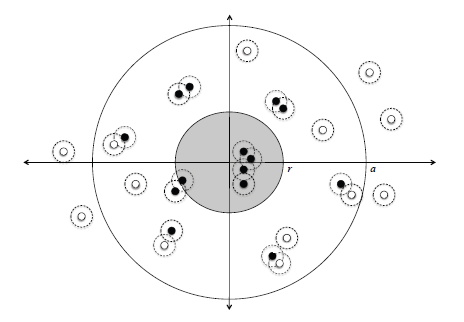
\includegraphics[width=0.6\textwidth]{img/anchor_zone}
 \caption{Moving nodes inside across an anchor zone. Black nodes are
 information-carrying nodes, white nodes will eventually get the information
 from the black ones. The probability of a node carrying an item tends to 1
 inside the replication zone, and decreases until reaching an availability a
 after which no more copies are found. }
 \label{fig:anchor_zone}
\end{figure}

The idea of the concept is that if two nodes meet in the anchor zone of some
information, and one of them doesn't have it stored in the data storage then the
other node will immediately send it so both nodes can be able to access it. As a
result, every node inside the anchor zone should have a copy of the item while
nodes which are leaving the anchor can delete it at their own discretion.

Let's consider two nodes A and B which encounter at some point in time. Node A
does have an item I tagged with an anchor zone centered in point P and radii
{\it a} and {\it r}. Let {\it h} be the distance of node A from the center P.
When node A meets node B, item I gets replicated to B with the probability
$p_r(h)$:

$$p_r(h) = \begin{cases}
	1 & \text{if } h \leq r \\
	R\left(h\right) & \text{if } r < h \leq a \\
	0 & \text{otherwise} \\
\end{cases}$$

$R(h)$ is a decreasing function which determines the probability of replication
between the outer replication border and the availability border of the anchor
zone.
The deletion probability $p_d(h)$ is defined as with $D(h)$ in $[0, 1]$ :

$$p_d(h) = \begin{cases}
	0 & \text{if } h \leq r \\
	D\left(h\right) & \text{if } r < h \leq a \\
	1 & \text{otherwise} \\
\end{cases}$$

The node preserves the free space due to the deletion function. It follows the
first in, first out (FIFO) principle, deleting the oldest items first if there
is a need for free space.

The area between {\it replication range} and {\it availability range} acts as a
buffer zone, that prevents immediate deletion of items. It is beneficial
for nodes that leave the {\it replication range} for a short period of time,
preventing them performing deletion operation. Thus, after returning inside
{\it replication range}, they have the associated items preserved. Outside the
anchor zone, a node could delete specific items when meeting with other nodes,
or at a predefined timeout, checking if items are outside their zones or their
lifetime expired.

As \cite{percomfloatingcontent} did, for simplicity and more trackability, in
our evaluation there is no buffer zone, i.e. {\it r = a}, deletion and replication
function becoming useless in this case.

\subsection{Communication Protocol}

As described in \cite{percomfloatingcontent}, the floating content protocol,
also used in our evaluations, is an efficient and simple method to exchange
items between nodes. A message is identified by a message id $Id$, the anchor point
with the attributes described earlier $(P, r, a)$, and the lifetime $T$. The
header of the message is filled with these characteristics, and the message body
of size $s(I)$ is filled with the desired payload.

Below is the protocol which has 4 phases:

\begin{enumerate}[1.]
  \item Nodes keep sending neighbor discovery beacons to discover peers.
  \item When receiving a discovery beacon, the peer decides to send in return,
  its list of items that verifies the condition $p_r(h) > 0$, thus valid for
  replication. In this phase the list contains only the attributes of the items,
  keeping this message as compact as possible: $Id$, $s(I)$, $(P, r, a)$ and
  lifetime $T$. If the list doesn't fit into a single message, it will be spread
  across multiple summary messages in a round-robin fashion.
  \item When receiving the list of items from a discovered peer, the node
  request those items for which $p_r(h)$ suggests that they should be replicated.
  \item In the last phase, requested items are exchanged until transfer
  completion or nodes lose contact. Upon this step, the protocol should remove
  uncompleted messages and return to phase 2.
\end{enumerate}

It is assumed that nodes can exchange messages fully bidirectional during any
step. Moreover, they can exchange messages simultaneously to multiple nodes
(even though technology may not be able). The beaconing process can take place
while in middle of message exchange in order to keep the discovering process
running. Since message exchanging is done in an incremental way, nodes can
append the new coming messages to the list, while they are still in transfer.

Deletion of item I occurs immediately the node moves outside of $a$. In
\cite{percomfloatingcontent} is is suggested that a second possibility could be
deletion $upon-encounter$ which discards a message when meeting a new node.
stating that this policy is more sensible due to its asynchronous
characteristic triggered by an external event. Naturally, deletion takes place
before the list of items is sent to other peers.

\subsection{Security issues and resource management}

The presented protocol does not restrict the user in any way, regarding content
generation and its context parameters. The single requirement is that the owner
must be in the anchor zone at the time of creation. In consequence, this may
represent a flaw in the protocol, users being able to insert items in network
with an infinite anchor zone. Flooding items represent a threat for the network,
because they exhaust the system resources very quickly, especially channel and
buffer capacity.

Reputation mechanisms like \cite{reputation} or accounting could represent
solutions to the above spamming issues. But it would be very difficult to
implement them without having an central infrastructure to enhance
authentication of identities. Also being a best-effort service is another nail
in the coffin for the rewarding system. Some simple mechanisms could be added to
implementation like prioritizing items taking into consideration their expected
storage consumption and the distance from the anchor. Thus, deleting the
farthest or the most largest item may discourage unlimited content distribution.

As shown in \cite{percomfloatingcontent}, the application can smartly manage its
resources by giving preference to items with smallest anchor range. Items with
very large anchor zones would have low availability due to the poor coverage it
may have. Of course a spammer could move around on a large area to create items
with small anchor zones and simulate an large anchor zone. There is no
prevention mechanism for this, but it is considered that the spammer should put
a lot of effort to achieve its goal. Also, the anchor zone needs to be
periodically revisited due to the ephemerality characteristic of the
information.
This security mechanism doesn't require infrastructure service or any degree of
mutual trust which is an advantage.


\section {Analytical model}

Floating content model has been a subject of analysis in
\cite{whendoesdatafloats} . The most important objective of this work has been
finding a pattern to guarantee that a specific information remains in its anchor
zone until the expiry of its lifetime with a high probability. It is called the
$criticality condition$ and it depends on many aspects like mobility pattern and
the replication policy of the nodes inside the anchor zone. 

\subsection{Criticality Condition}

As before, we assume each information is being tagged with an anchor zone in
which nodes keep entering, spend some time and finally exit. Also, we assume
that the nodes spend a relatively long time inside the anchor and follow a
random mobility pattern. The population is assumed to be large and ``well
mixed'' in order to preserve the proportion between its size and the nodes
having the information. Further the criticality condition at the
fluid limit is explained.

While moving inside the anchor zone, a node encounters randomly other nodes.
We assume there are only two nodes moving permanently inside the zone. Let
$\upsilon$ be the frequency at which they come in contact with each other. Now,
assuming the population of nodes in anchor is N, then the total number of pairs
is $\frac{1}{2}N(N-1) \approx \frac{1}{2}N^2$ and the total rate of encounters
is $\frac{1}{2}N^2\upsilon$. A part of these encounters, more exactly $2p(1-p)$,
replicate an item to nodes that doesn't have it yet in the data storage, thus
the total rate of such events is $p(1-p)N^2\upsilon$. At this rate, the size of
the population of nodes which have the item I tends to increase. Let
$\frac{1}{\mu}$ be the time spent by a node in the anchor zone. It results that
the total exit rate of nodes is $N\mu$ and the exit rate of tagged nodes is
$Np\mu$. The growth rate is determined by the formula:

\begin{equation}
N\frac{d}{dt}p = N^2p(1-p)\upsilon - Np\mu \label{eq:derivative}
\end{equation}

The two terms on the right hand side are equal in equilibrium leading to the
stationary value $p^* = 1 - \mu / (\upsilon N)$. In order to have a positive
solution, $p^* > 0$, it requires that,

\begin{equation}
N\frac{\upsilon}{\mu} > 1. \label{eq:criticality}
\end{equation}

Equation \eqref{eq:criticality} is called {\it criticality condition}. The left
hand side value represents the average number of collisions a randomly chosen
node has during its sojourn time. Taking into consideration the sign of
the equation \eqref{eq:derivative} it can be seen that the solution is stable.
If $p > 1 - \mu / (\upsilon N)$ it tends to increase, else if $p < 1 - \mu /
(\upsilon N)$ it tends to decrease. The information disappears (even in the
fluid model) when the derivative is everywhere negative leading the solution to
p = 0. Moreover, since we need to prevent accidental disappearance of the
information carrying population by stochastic fluctuations, $Np = N - \mu /
\upsilon$ must be large.

\subsection{Model applicability}

It can be seen that the black non-spatial model for content exchange is highly
abstract, only capturing the essential elements. The most important assumptions
on which the model relies on are the fluid limit approximation and a well-mixed
mobility pattern. In this case the criticality condition shows that the
information ``floats'' due to the large number of nodes in the anchor zone
assumed by the fluid limit approximation. In a real case situation the number of
nodes carrying the information may be small, thus having a big probability of
information disappearance due to stochastic fluctuations in the system. The well
mixed characteristic of the population leads to the fact that all the nodes
inside an anchor zone, are equally likely to encounter each other at some point
of time, past encounters having no influence on it.

In my simulation, which will be discussed later in the document, the spatial
aspects of information exchange is ignored. So the probability of a node
carrying information is the same on the entire simulation network (of course
without taking in consideration water zones). In addition, the criticality
condition doesn't take into consideration some important parameters. On of the
would be the transmission range which affects directly the encounter rate
$\upsilon$.

The non-spatial model is applied in the simulation performed, because it
captures the fundamental elements of the system, and defines the criticality
condition which is an indicator whether an information item may float or not. As
in \cite{percomfloatingcontent} we compute three key elements and then observe
how the criticality condition correlates with the road network and the final
information life time. The simulation results happened to be very similar,
confirming the applicability of the abstract model in complex mobility
scenarios.

%\newpage
%\thispagestyle{plain}

\end{document}
% ==== END OF BODY =============================================================